\documentclass[tikz]{standalone}
\usetikzlibrary{positioning, arrows.meta}
\begin{document}
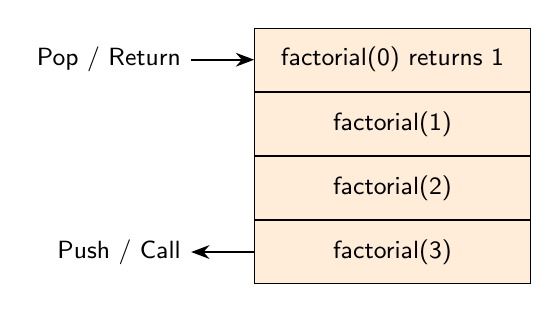
\begin{tikzpicture}[
    frame/.style={rectangle, draw, minimum width=3.5cm, minimum height=0.8cm, fill=orange!15, font=\sffamily\small}
]
    \node[frame] (f1) {factorial(0) returns 1};
    \node[frame, below=0cm of f1] (f2) {factorial(1)};
    \node[frame, below=0cm of f2] (f3) {factorial(2)};
    \node[frame, below=0cm of f3] (f4) {factorial(3)};

    \draw[{Stealth}-, thick] (f1.west) -- ++(-0.8,0) node[left, font=\sffamily\small] {Pop / Return};
    \draw[-{Stealth}, thick] (f4.west) -- ++(-0.8,0) node[left, font=\sffamily\small] {Push / Call};

\end{tikzpicture}
\end{document}